\section{Data Description}
\label{sec:data}

\subsection{Data Source and Collection}
\label{sec:data_source}

Our data were obtained from Swing, one of the largest shared e-scooter operators in South Korea. As of 2023, Swing operated fleets of electric scooters and electric bicycles across more than 50 cities nationwide, serving hundreds of thousands of active users per month. Swing provided two complementary datasets for this research under a data sharing agreement:

\begin{enumerate}
    \item \textbf{Trajectory dataset} (May 2023): 2,830,461 trip records, each containing the full GPS route as a sequence of latitude-longitude-timestamp triples recorded at approximately 10-second intervals, along with a per-trip speed vector (\texttt{speeds}) recording instantaneous speed readings from the vehicle's onboard sensor at each GPS recording point. This dataset also includes trip metadata such as vehicle model, operating mode, travel time, distance, and start/end coordinates.

    \item \textbf{Trip-level dataset} (January--October 2023): 20,045,245 trip records with user demographics (anonymized \texttt{user\_id}, \texttt{age}), vehicle characteristics (\texttt{vehicletype}, \texttt{smodel}, \texttt{mode}), billing information (\texttt{bill\_amt}, \texttt{disc\_amt}), and temporal attributes (\texttt{date}, \texttt{start\_time}, \texttt{end\_time}). This dataset does not contain GPS trajectories or speed profiles but provides demographic and usage variables for the broader user population.
\end{enumerate}

The two datasets can be linked via the shared \texttt{user\_id} field, enabling us to merge trajectory-level speed behavior with user-level demographic information. All user identifiers were anonymized by the operator prior to data transfer, and no personally identifiable information was included.

For the longitudinal experience analysis (Section~\ref{sec:res_experience}), we additionally use 24 monthly trajectory files spanning January 2022 through December 2023, containing a total of 47.0~million raw trips (44.1~million after quality filtering) from 1,816,911 unique users. These monthly files include the same schema as the May 2023 trajectory dataset but with an important caveat: the speed sensor data (\texttt{avg\_speed}, \texttt{max\_speed}, \texttt{speeds}) are only available from February 2023 onward. Earlier months (all of 2022 and January 2023) contain sentinel values ($-999$) for all speed columns. These trips are retained for user longitudinal tracking---computing cumulative trip ranks and experience measures---but are excluded from speeding outcome analysis.

\subsection{Data Schema and Key Variables}
\label{sec:data_schema}

Table~\ref{tab:data_summary} summarizes both datasets. The trajectory dataset contains 25 columns. Two variables are central to our analysis. The \texttt{speeds} column stores a nested list of integer speed readings (km/h) from the onboard sensor at each GPS point; we verified that \texttt{max\_speed} exactly equals the maximum of this array ($r = 1.0$). The \texttt{routes} column stores the GPS trajectory as \texttt{[latitude, longitude, timestamp]} triples.

Four scooter models appear after filtering: S9 (75.9\%), W9 (11.4\%), S11 (6.3\%), and S7 (5.1\%); the I9 moped model (0.4\%) was excluded. The \texttt{mode} field records the operating mode: TUB (turbo, no speed limit), STD (standard, $\sim$20~km/h), and ECO (economy, $\sim$15~km/h). Bicycle modes (BIKE\_TUB, BIKE\_STD) account for 11.3\% of trips. Crucially, all modes use identical hardware---only the software-based speed limit differs.

\subsection{Data Quality and Preprocessing}
\label{sec:data_quality}

We applied a multi-stage quality filtering pipeline (Table~\ref{tab:filtering}), removing I9 moped trips (0.37\%), replacing sentinel values ($-999$ for NULL; 0.74\%), excluding invalid GPS coordinates outside Korea (0.006\%), trips with $< 5$ GPS points (1.23\%), and implausible maximum speeds $> 50$~km/h (0.24\%). After core filtering, 2,780,890 valid trips remained (98.2\% retention). A strict-filtered subset (2,664,263 trips; 94.1\%) additionally excludes short-distance ($< 100$~m), short-duration ($< 60$~s), and excessive-duration ($> 7{,}200$~s) trips for sensitivity analyses.

\begin{table}[htbp]
\centering
\caption{Multi-stage quality filtering pipeline applied to the trajectory dataset.}
\label{tab:filtering}
\small
\begin{tabular}{clr}
\toprule
\textbf{Stage} & \textbf{Filter criterion} & \textbf{Flagged trips} \\
\midrule
--- & Raw dataset & 2,830,461 (total) \\
1 & I9 model (moped class) & 10,556 (0.37\%) \\
2 & Sentinel value $-999$ replacement$^*$ & 20,844 (0.74\%) \\
3 & Invalid GPS coordinates & 162 (0.006\%) \\
4 & $< 5$ GPS points & 34,820 (1.23\%) \\
5 & Max speed $> 50$ km/h & 6,790 (0.24\%) \\
\addlinespace
& \textbf{Excluded by any core filter$^\dagger$} & \textbf{49,571 (1.75\%)} \\
& \textbf{Valid trips (core filters)} & \textbf{2,780,890 (98.2\%)} \\
\addlinespace
\multicolumn{3}{l}{\textit{Additional quality flags (not excluded from primary analysis)}} \\
6 & Distance $< 100$ m & 110,456 (3.97\%) \\
7 & Duration $< 60$ s & 57,813 (2.08\%) \\
8 & Duration $> 7{,}200$ s & 1,210 (0.04\%) \\
\addlinespace
& \textbf{Strict-filtered dataset} & \textbf{2,664,263 (94.1\%)} \\
\bottomrule
\multicolumn{3}{l}{\footnotesize $^*$Sentinel values replaced, not removed; count reflects affected trips.} \\
\multicolumn{3}{l}{\footnotesize $^\dagger$Filters 1, 3--5 applied simultaneously; some trips flagged by multiple filters.} \\
\end{tabular}
\end{table}

To validate sensor reliability, we compared onboard speeds against GPS-derived speeds on 9,884 trips. Sensor-derived averages agree well with reported \texttt{avg\_speed} ($r = 0.844$, MAE $= 1.65$~km/h), while GPS-derived maximum speeds show poor correlation ($r = 0.138$) due to the $\sim$10-second sampling interval attenuating peak speeds. We therefore use onboard sensor speeds throughout.

\subsection{City Assignment and Geographic Coverage}
\label{sec:data_cities}

Trip origins were assigned to cities using a KD-tree nearest-neighbor approach with 54 Korean city centers. The final dataset spans 52 cities across all 17 provinces (Table~\ref{tab:city_coverage}). The Seoul Capital Area accounts for 63.1\% of trips; Seoul alone contributes 577,133 trips (20.8\%), followed by Daejeon (5.5\%) and Suwon (4.8\%). All seven metropolitan cities are represented. Figure~\ref{fig:spatial_distribution} maps trip origins with speeding rate by color.

\subsection{Descriptive Statistics}
\label{sec:data_descriptive}

The final dataset comprises 2,780,890 valid trips by 382,328 users across 81,525 vehicles (May 2023), with age data available for 90.4\% of users (median 25, mean 28 years). Table~\ref{tab:data_summary} summarizes key statistics. The overall speeding rate is 29.6\%, but this masks heterogeneity: 60.9\% of users never speed, while 17.3\% speed on over half their trips.

Among 2,323,154 scooter-mode trips, TUB accounts for 55.0\%, STD 40.2\%, and ECO 4.8\%.\footnote{Trips with mode ``none'' (5.2\%, primarily S7 model in Ulsan) are excluded from mode-specific analyses.} Speed profiles differ dramatically: TUB mode shows a 54.0\% speeding rate versus 0.9\% (STD) and 1.1\% (ECO). Temporal patterns show bimodal daily peaks (morning commute and evening) with slightly elevated speeding during late-night hours.

% === TABLES ===

\begin{table}[htbp]
\centering
\caption{Summary statistics of the trajectory dataset (May 2023) and the trip-level dataset (January--October 2023).}
\label{tab:data_summary}
\small
\begin{tabular}{llrr}
\toprule
\textbf{Attribute} & \textbf{Unit} & \textbf{Trajectory Dataset} & \textbf{Trip-Level Dataset} \\
\midrule
Total records & trips & 2,830,461 & 20,045,245 \\
Valid records (after filtering) & trips & 2,780,890 & --- \\
Retention rate & \% & 98.2 & --- \\
Unique users & --- & 382,328 & 1,892,415$^*$ \\
Unique vehicles & --- & 81,525 & --- \\
Date coverage & & May 2023 & Jan--Oct 2023 \\
\addlinespace
\multicolumn{4}{l}{\textit{Trip characteristics (trajectory dataset, valid trips)}} \\
\addlinespace
Mean distance & m & 878 & --- \\
Mean duration & s & 377 & --- \\
Mean GPS points per trip & --- & 37.8 & --- \\
Mean GPS interval & s & 10.1 & --- \\
\addlinespace
\multicolumn{4}{l}{\textit{Speed characteristics (trajectory dataset, valid trips)}} \\
\addlinespace
Mean average speed & km/h & 13.9 & --- \\
P85 average speed & km/h & 18.6 & --- \\
Mean maximum speed & km/h & 22.9 & --- \\
Speeding rate (max $> 25$ km/h) & \% & 29.6 & --- \\
\addlinespace
\multicolumn{4}{l}{\textit{User demographics (trip-level dataset)}} \\
\addlinespace
Mean age & years & --- & 28 \\
Median age & years & --- & 25 \\
Age data availability & \% & --- & 90.4 \\
\bottomrule
\multicolumn{4}{l}{\footnotesize $^*$Estimated from the full 10-month dataset.} \\
\end{tabular}
\end{table}

\begin{table}[htbp]
\centering
\caption{Geographic distribution of valid trips across the top 20 cities (of 52 total).}
\label{tab:city_coverage}
\small
\begin{tabular}{llrrr}
\toprule
\textbf{City} & \textbf{Province} & \textbf{Trips} & \textbf{Share (\%)} & \textbf{Cumulative (\%)} \\
\midrule
Seoul & Seoul & 577,133 & 20.75 & 20.75 \\
Daejeon & Daejeon & 154,075 & 5.54 & 26.29 \\
Suwon & Gyeonggi & 133,223 & 4.79 & 31.08 \\
Seongnam & Gyeonggi & 126,542 & 4.55 & 35.63 \\
Bucheon & Gyeonggi & 125,018 & 4.50 & 40.13 \\
Anyang & Gyeonggi & 120,707 & 4.34 & 44.47 \\
Osan & Gyeonggi & 112,541 & 4.05 & 48.52 \\
Busan & Busan & 96,273 & 3.46 & 51.98 \\
Cheonan & Chungnam & 89,778 & 3.23 & 55.21 \\
Daegu & Daegu & 84,556 & 3.04 & 58.25 \\
Ulsan & Ulsan & 81,987 & 2.95 & 61.20 \\
Jeonju & Jeonbuk & 81,036 & 2.91 & 64.11 \\
Incheon & Incheon & 58,024 & 2.09 & 66.20 \\
Ansan & Gyeonggi & 50,818 & 1.83 & 68.03 \\
Icheon & Gyeonggi & 48,338 & 1.74 & 69.77 \\
Hwaseong & Gyeonggi & 45,097 & 1.62 & 71.39 \\
Gimpo & Gyeonggi & 45,027 & 1.62 & 73.01 \\
Siheung & Gyeonggi & 44,477 & 1.60 & 74.61 \\
Pyeongtaek & Gyeonggi & 42,646 & 1.53 & 76.14 \\
Cheongju & Chungbuk & 42,580 & 1.53 & 77.67 \\
\addlinespace
\multicolumn{2}{l}{\textit{Remaining 32 cities}} & 621,014 & 22.33 & 100.00 \\
\midrule
\textbf{Total} & & \textbf{2,780,890} & \textbf{100.00} & \\
\bottomrule
\end{tabular}
\end{table}

\begin{figure}[htbp]
\centering
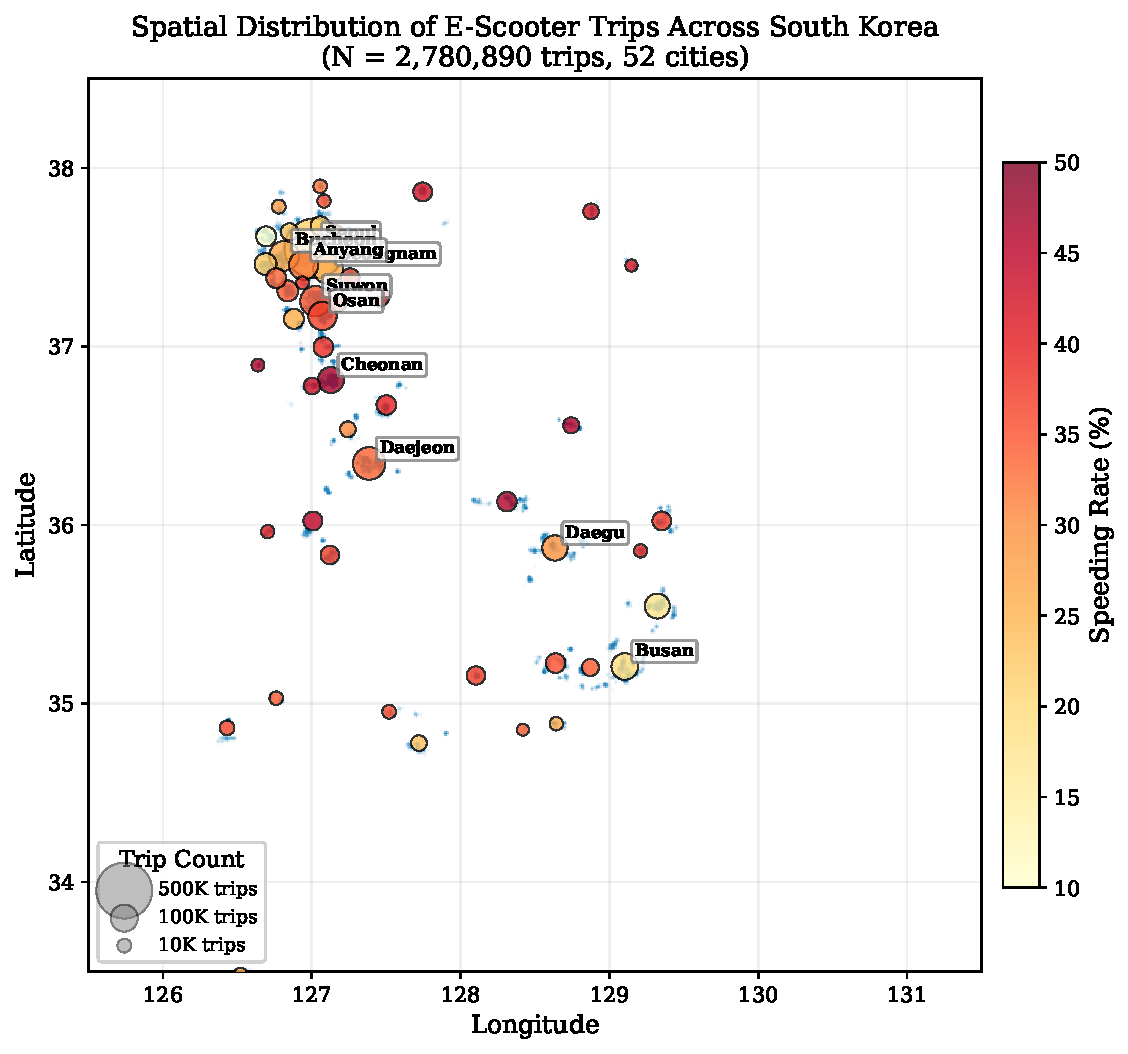
\includegraphics[width=\textwidth]{figures/fig1_spatial_distribution.pdf}
\caption{Spatial distribution of trip origins across Korean cities. Bubble size indicates trip volume; color indicates mean speeding rate. Labels show the top 10 cities by trip count.}
\label{fig:spatial_distribution}
\end{figure}

\begin{figure}[htbp]
\centering
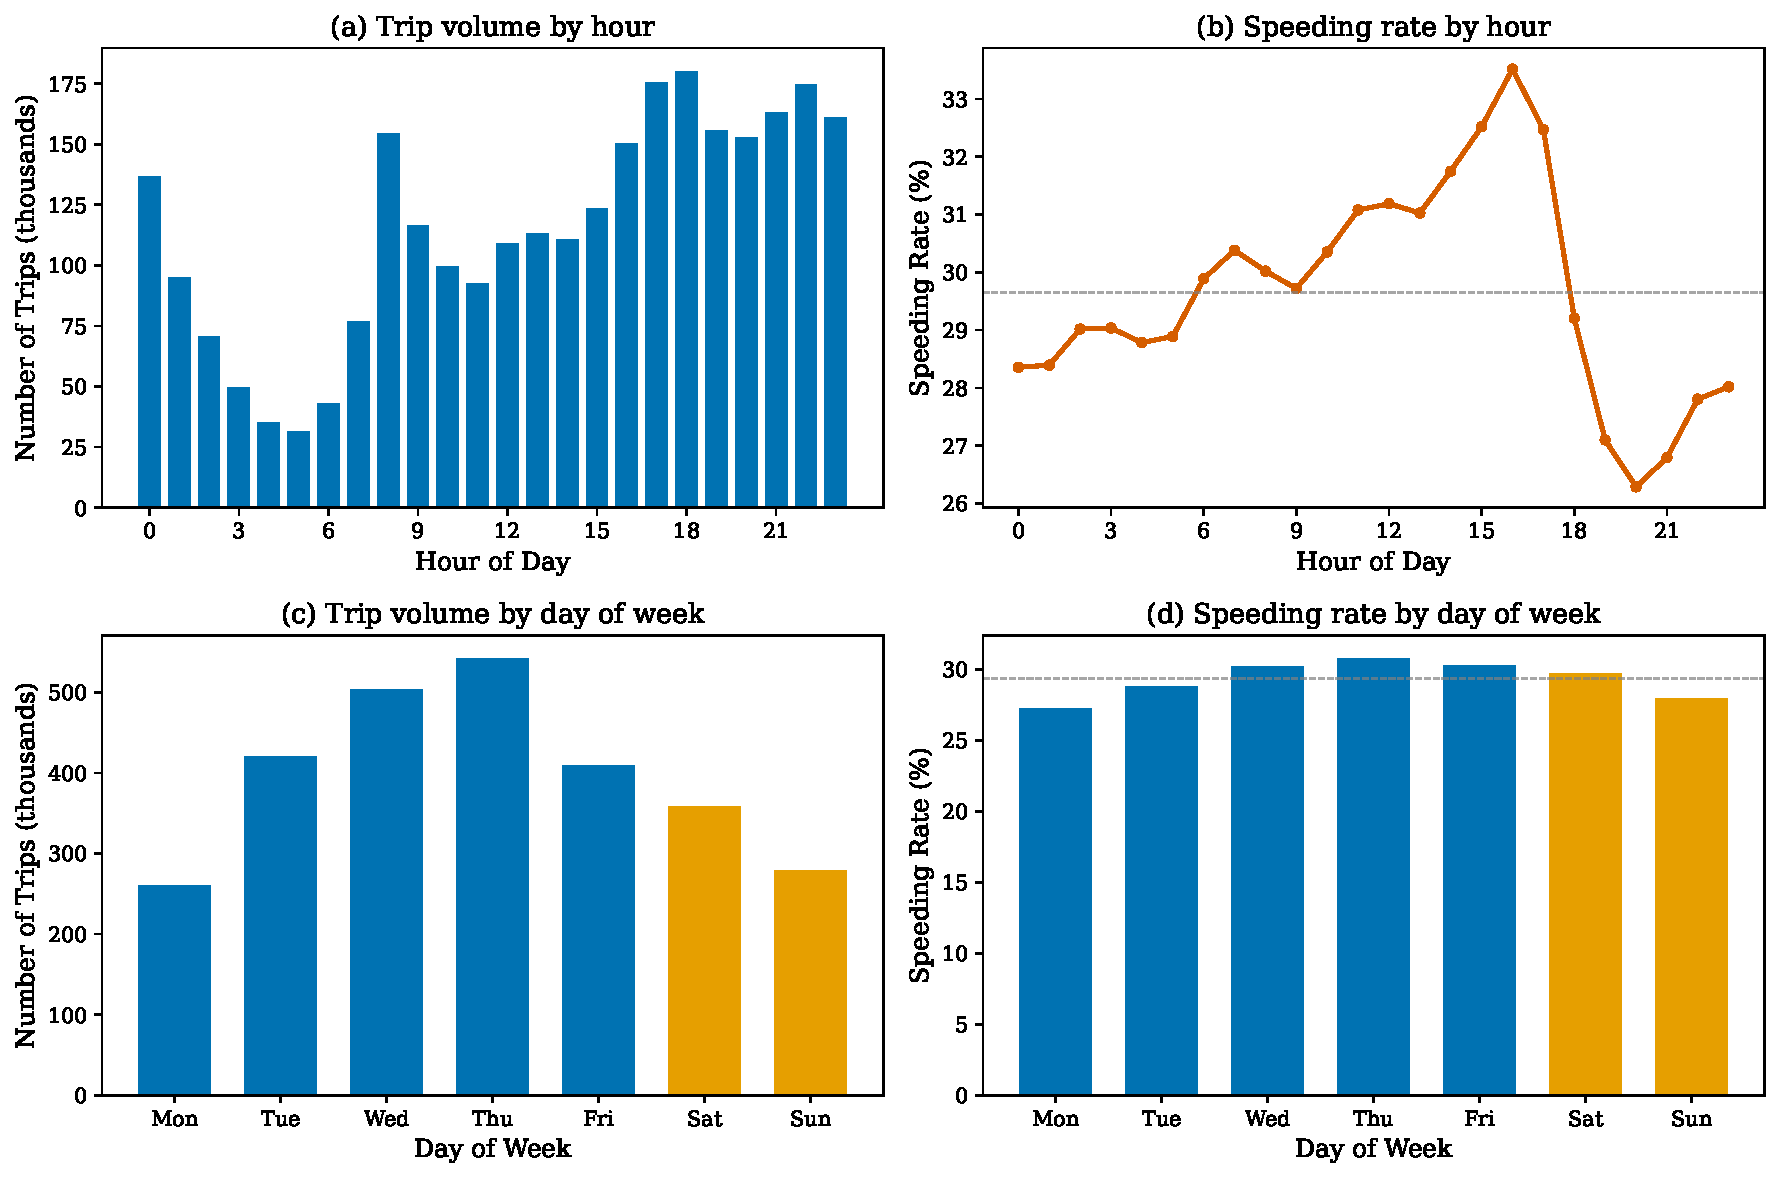
\includegraphics[width=\textwidth]{figures/fig2_temporal_distributions.pdf}
\caption{Temporal distributions of trip volume and speeding rate: (a) by hour of day and (b) by day of week. Blue bars indicate trip counts (left axis); red lines indicate the speeding rate (right axis).}
\label{fig:temporal}
\end{figure}
